\chapter{Обзор литературы}\label{ch:ch1}

\section{Исследование композитных материалов}\label{sec:ch1/sec1}

Пьезоэлектрические устройства используются для преобразования механической энергии в электрическую и наоборот. Такие устройства применяются в технологиях для получения и накопления энергии, в различных медицинских приборах, при разработке систем, работающих в жидких и акустических средах. Рабочим элементом пьезопреобразователя является пьезокерамический элемент определенной формы. Форма и тип деформации этого элемента определяют пьезомодули, которые характеризуют преобразование механической энергии деформации в электрическую. Так пьезомодуль $d33$ связан с растяжением-сжатием вдоль оси поляризации, $d31$~--- с такой же деформацией в поперечном направлении к этой оси, $d15$~--- со сдвигом. Использование пористой керамики позволяет создавать более эффективные пьезопреобразователи. Очевидным преимуществом является уменьшение веса, но также необходимо учитывать жесткость и, что самое важное, выходной потенциал. В случае пористой керамики модули упругости с ростом пористости убывают значительно сильнее, чем пьезомодули, то есть при одной и той же механической нагрузке амплитуда деформации у пористой керамики будет больше, а следовательно и выходной электрический потенциал тоже  растет. 

Задача поиска оптимального дизайна таких устройств требует учета как геометрических характеристик отдельных частей устройства, так и подбора материалов со свойствами, подходящими для определенных режимов колебаний.

Актуальность исследований в данной области подтверждается интересом различных групп исследователей к задачам оптимизации пьезоэлектрических устройств. В работе~\cite{Yu2016} решается задача оценки эффективности электромеханической связи в режиме сдвига-изгиба для пьезоэлектрической пластины кольцевой формы. В соответствии с классической теорией упругих пластин малого изгиба и пьезоэлектрическими определяющими соотношениями получено аналитическое решение для изгибной деформации преобразователя под действием электрического поля и концентрированной или равномерно распределенной механической нагрузки. Определено оптимальное соотношение внутреннего и внешнего радиусов. В работе~\cite{Gao2018} рассмотрен многослойный цилиндрический пьезопреобразователь~(MCPSA), работающий в режиме сдвига~$d_{15}$. Устройство состоит из пьезокерамических колец, концентрически собранных вместе с попеременной положительной и отрицательной поляризацией в осевом направлении. Проведены эксперименты, исследованы характеристики смещения устройства при приложенном напряжении и механической нагрузке. Статья~\cite{Yan2018} посвящена исследованию многослойных пьезоэлектрические преобразователей с акцентом на высокую выходную мощность. Целью исследования является создание повышение плотности мощности устройства. В работе~\cite{Yang2019} рассматривается процесс создания дизайн нового пьезоэлектрического метаматериала. На основе этого материала разработаны многослойные структуры, работающие в сдвиговом режиме.

Сдвиговые колебания устройств из пьезокерамики широко используются в прикладной технике. Сбор энергии - один из основных способов использования таких материалов~\cite{Mohanty2019, Elahi2018, Almanza2023}, поскольку он позволяет собирать <<зеленую>> энергию с низкой стоимостью. Известны ограничения этого подхода, включая деградацию керамики после некоторого времени использования или ограниченное напряжение, но новые пьезоматериалы позволяют создавать не только традиционные крупномасштабные сборщики энергии, но и небольшие носимые устройства. Такие материалы также актуальны при нанообработке~\cite{Xue2022}.

Поведение упругих и электроупругих тел описывается следующими уравнениями и определяющими соотношениями:
\begin{equation} \label{eq_solid:1}  
\begin{aligned} 
	\begin{array}{ll} 
		\rho_{j} \omega^2 \boldsymbol{\ddot u}+\alpha_{dj}\rho_j\boldsymbol{\dot u}-\nabla \cdot \boldsymbol{\sigma} =\boldsymbol{f_{j}}; & \nabla \cdot \boldsymbol{D}={0};\\ 
		\boldsymbol{\sigma} =\boldsymbol{c_{j}^{E}} \cdot \cdot (\boldsymbol{\varepsilon}+\beta_{dj}\boldsymbol{\dot \varepsilon})-\boldsymbol{e_{j}^{T}} \cdot \boldsymbol{E}; & \boldsymbol{E}=-\nabla \varphi;\\
		\boldsymbol{D}+\varsigma_{dj}\boldsymbol{\dot {D}} =\boldsymbol{e_{j}} \cdot \cdot  \boldsymbol{\varepsilon}+\boldsymbol{k_{j}} \cdot \boldsymbol{E}; & \boldsymbol{\varepsilon} =(\nabla \boldsymbol{u}+\nabla \boldsymbol{u}^{T} )/2\\
	\end{array} 
\end{aligned}
\end{equation}
где
$\boldsymbol{\sigma}$~--- тензор напряжений,
$\rho$~--- плотность, 
$\boldsymbol{\varepsilon}$~--- тензор деформаций,
$\boldsymbol{u}$~--- вектор перемещений,
$\boldsymbol{D}$~--- вектор электрической индукции,
$\boldsymbol{E}$~--- вектор напряженности электрического поля,
$f$~--- вектор массовых сил,
$\varphi$~--- электрический потенциал,
$\boldsymbol{c}^{E}$~--- тензор упругих констант,
$\boldsymbol{e}^{T}$~--- тензор пьезомодулей,
$\boldsymbol{k}$~--- тензор диэлектрических проницаемостей,
$\omega$~--- круговая частота,
$\alpha_d, \beta_d, \varsigma_d$~--- коэффициенты демпфирования,
$j$~--- номер тела в моделе.

На основе первых уравнений (\ref{eq_solid:1}) конечно-элементную модель в векторной форме записывается следующим образом:
\begin{equation}\label{eq:2}
\begin{aligned}  
	\boldsymbol{u}(\boldsymbol{x},t)=\boldsymbol{N}_{u}^{T}(\boldsymbol{x}) \cdot \boldsymbol{U}(t);\\
	\varphi(\boldsymbol{x},t)=\boldsymbol{N}_{\varphi }^{T}(\boldsymbol{x})\cdot \boldsymbol{\Phi}(t)
\end{aligned} 
\end{equation}
где $\boldsymbol{N}_{u}$-- матрица функций формы для поля перемещений, $\boldsymbol{N}_{\varphi }^{} $-вектор функций формы для электрического потенциала. $\boldsymbol{U}\left(t\right),\, \, \boldsymbol{\Phi} \left(t\right)$-- глобальные векторы соответствующих узловых степеней свободы.


\subsection{Идентификация материала}

Для определения материальных свойств композитных материалов применяется метод осреднения~\cite{Do2023}. В основе этого метода лежит идея вычисления средних свойств материала для представительных объемов. После того как все свойства известны, модель материала может быть сведена к общему анизотропному электроупругому материалу.

%Метод эффективных модулей реализованный в пакете ACELAN--COMPOS позволяет полностью учесть внутреннюю структуру пористого пьезоэлектрического композиционного материала, включая типы связности, размеры пор и различные локальные эффекты. 

Для определения свойств материала в представительном объеме $V$ решается статическая задача электроупругости со специальными граничными условиями.
Система уравнений в объеме получается из~(\ref{eq_solid:1}) для функций $u$ и $\phi$, которые зависят только от пространственной координаты~$x$. Тогда уравнения~(\ref{eq_solid:1}) можно записать в виде:

\begin{equation} \label{eq_solid:2}  
	\begin{aligned}
	\begin{array}{ll} 
		\nabla \cdot \boldsymbol{\sigma} =0; & \nabla \cdot \boldsymbol{D}={0};\\ 
		\boldsymbol{\sigma} =\boldsymbol{c}^{E} \cdot \cdot \boldsymbol{\varepsilon}-\boldsymbol{e}^{T} \cdot \boldsymbol{E}; & \boldsymbol{E}=-\nabla \varphi;\\
		\boldsymbol{D} =\boldsymbol{e} \cdot \cdot  \boldsymbol{\varepsilon}+\boldsymbol{k} \cdot \boldsymbol{E} & \boldsymbol{\varepsilon} =(\nabla \boldsymbol{u}+\nabla \boldsymbol{u}^{T} )/2.\\
	\end{array} 
\end{aligned} 
\end{equation}

Граничные условия в задаче усреднения  пористого пьезокомпозитного материала~\cite{Mawassy2021} используются:  

\begin{equation}\label{eq_solid:3} 
	\begin{aligned}
	\boldsymbol{u}=\boldsymbol{x} \cdot \boldsymbol{\varepsilon}_0, \quad \phi=-\boldsymbol{x} \cdot \boldsymbol{E}_0, \quad \boldsymbol{x} \in \Gamma=\partial V,
\end{aligned} 
\end{equation}
где $\boldsymbol{\varepsilon_0}=\boldsymbol{\varepsilon_0^T}$~--- симметричный тензор постоянных деформаций второго ранга, $\boldsymbol{E_0}$~--- постоянный вектор электрического поля.

Для однородной среды решением краевой задачи~(\ref{eq_solid:2}), (\ref{eq_solid:3}) является $\boldsymbol{u}=\boldsymbol{x} \cdot \boldsymbol{\varepsilon}_0$, $\phi=-\boldsymbol{x} \cdot \boldsymbol{E}_0$ с постоянными эффективными модулями.

Для решения краевой задачи~(\ref{eq_solid:2}), (\ref{eq_solid:3}) в неоднородродном объеме $V$:

\begin{equation}\label{eq2:1} 
	\begin{aligned}
	<\boldsymbol{\varepsilon}>=\boldsymbol{\varepsilon}_0^T, \quad <\boldsymbol{E}>=\boldsymbol{E}_0,
\end{aligned} 
\end{equation}
где $<\bullet>=\frac1{|V|}\int_V(\bullet)dV$~--- усредненные по объему значения.

Условиями определения эффективных модулей являются соотношения $<\boldsymbol{\sigma}>=\boldsymbol{\sigma}_0$, $<\boldsymbol{D}>=\boldsymbol{D}_0$. Эти равенства позволяют получить полный набор эффективных модулей пьезокомпозиционного материала из решения серии краевых задач~(\ref{eq_solid:2}), (\ref{eq_solid:3}) с различными ненулевыми компонентами в $\boldsymbol{\varepsilon}_0$ и $\boldsymbol{E}_0$.

Для определения полного набора констант для пьезокомпозитного материала необходимо решить~9 краевых задач~(\ref{eq_solid:2}) с граничными условиями~(\ref{eq_solid:3}): 6 задач, если 

\[
\begin{aligned}
\boldsymbol{\varepsilon}_0=S_0(\boldsymbol e_k \boldsymbol e_m+ \boldsymbol e_m \boldsymbol e_k)/2, \quad \boldsymbol{E}_0=0,
\end{aligned} 
\]
и 3 задачи, если
\[
\begin{aligned}
\boldsymbol{\varepsilon}_0=0, \quad \boldsymbol{E}_0=E_0\boldsymbol e_k,
\end{aligned} 
\]
где $k,m=(1,2,3)$~--- зафиксированные индексы, $\boldsymbol e_k$, $\boldsymbol e_m$~--- единичные векторы декартова базиса, $S_0=const$, $E_0=const$.

Получаются следующие эффективные модули:
\[
\begin{aligned}
c_{ijkm}^{E,eff}=<\sigma_{ij}/S_0, \quad
e_{jkm}^{eff}=<D_j>/S_0,
\end{aligned} 
\]
\[
\begin{aligned}
e_{kij}^{eff}=-<\sigma_{ij}>/E_0, \quad
\kappa_{jk}^{S,eff}=<D_j>/E_0.
\end{aligned} 
\]

Для записи свойств материала используется матричная нотация Фойгта:

\[ 
\begin{aligned}
\boldsymbol{c}^E=
\begin{bmatrix}
	c_{11}^E & c_{12}^E & c_{13}^E & 0 & 0 & 0 \\ 
	c_{12}^E & c_{11}^E & c_{13}^E & 0 & 0 & 0 \\ 
	c_{13}^E & c_{13}^E & c_{33}^E & 0 & 0 & 0 \\ 
	0 & 0 & 0 & c_{44}^E & 0 & 0 \\
	0 & 0 & 0 & 0 & c_{55}^E & 0 \\
	0 & 0 & 0 & 0 & 0 & c_{66}^E\\
\end{bmatrix}, \quad
\boldsymbol{e}^T=
\begin{bmatrix}
	0 & 0 & e_{31} \\
	0 & 0 & e_{31} \\
	0 & 0 & e_{33} \\
	0 & e_{15} & 0 \\
	e_{15} & 0 & 0 \\
	0 & 0 & 0 \\
\end{bmatrix}, 
\end{aligned} 
\]

% \[
% \bm{D}=
% \begin{bmatrix}
	% 0 & 0 & 0 & 0 & d_{15} & 0 \\
	% 0 & 0 & 0 & d_{15} & 0 & 0\\
	% d_{31} & d_{31} & d_{33} & 0 & 0 & 0 \\
	% \end{bmatrix}, 
% \]


\[
\begin{aligned}
\boldsymbol{k}^S=
\begin{bmatrix}
	k^S_{11} & 0 & 0 \\
	0 & k^S_{11} & 0 \\
	0 & 0 & k^S_{33} \\
\end{bmatrix}, 
\end{aligned} 
\]
где $c_{66}^E=(c_{11}^E-c_{11}^E)/2$.
Значения тензоров переводятся в значения матриц по следующему правилу: $\alpha, \beta =1 \dots 6$, $i,j,k,m = 1,2,3$, $c^E_{\alpha \beta}=c^E_{ijkm}$, $\alpha \leftrightarrow (ij)$, $\beta \leftrightarrow (km)$, 
$1 \leftrightarrow (11)$, 
$2 \leftrightarrow (22)$, 
$3 \leftrightarrow (33)$, 
$4 \leftrightarrow (23)$,
$5 \leftrightarrow (13)$,
$6 \leftrightarrow (12)$.

%Полученные в пакете ACELAN--COMPOS эффективные модули для пьезокомпозитной керамики с типом связности~3-0 представлены в таблице~\cite{Nasedkin2020}~\ref{t:1}.
%\begin{table}[H]    \centering
%	\caption{Material properties}\label{t:1}
%	\begin{tabular}{|l|c|c|c|c|c|c|c|c|c|}
%		\hline
%		Porosity, \% &  0  & 10 & 20 & 30 & 40 & 50 &  60  & 70 & 80 \\ \hline
%		$\rho$, $kg/m^3$ &  7500  & 6750 & 6000 & 5250 & 4500 & 3750 & 3000 & 2250 & 1500 \\ \hline
%		$c_{11}^{E,eff}$, $10^{10}$,  & 13.9 & 11.56 & 9.25 & 6.85 & 5.05 & 3.34 & 2.07 & 1.26 & 0.68 \\ 
%		$N/m^2$ &  &  &  &  &  &  &  &  &  \\ \hline
%		$c_{12}^{E,eff}$, $10^{10}$, & 7.78 & 6.15 & 4.66 & 3.14 & 2.10 & 1.16 & 0.62 & 0.28 & 0.13 \\ 
%		$N/m^2$ &  &  &  &  &  &  &  &  &  \\ \hline
%		$c_{13}^{E,eff}$, $10^{10}$, & 7.43 & 5.82 & 4.25 & 2.82 & 1.87 & 1.06 & 0.52 & 0.24 & 0.1 \\ 
%		$N/m^2$ &  &  &  &  &  &  &  &  &  \\ \hline
%		$c_{33}^{E,eff}$, $10^{10}$, & 11.5 & 9.53 & 7.23 & 5.42 & 3.91 & 2.72 & 1.63 & 0.91 & 0.47 \\ 
%		$N/m^2$ &  &  &  &  &  &  &  &  &  \\ \hline
%		$c_{44}^{E,eff}$, $10^{10}$, & 2.56 & 2.23 & 1.83 & 1.44 & 1.10 & 0.74 & 0.44 & 0.23 & 0.1 \\ 
%		$N/m^2$ &  &  &  &  &  &  &  &  &  \\ \hline
%		$e_{33}^{eff}$, $C/m^2$ & 15.1 & 13.38 & 11.37 & 9.59 & 7.68 & 5.93 & 3.93 & 2.30 & 1.25 \\ \hline
%		$e_{31}^{eff}$, $C/m^2$ & -5.2 & -4.23 & -3.14 & -2.07 & -1.32 & -0.75 & -0.43 & -0.21 & -0.1 \\ \hline
%		$e_{51}^{eff}$, $C/m^2$ & 12.7 & 10.96 & 8.96 & 6.91 & 5.00 & 3.30 & 1.95 & 1.00 & 0.44 \\ \hline
%		$k_{11}^{S,eff}/\varepsilon_0$ & 730 & 663 & 582 & 509 & 439 & 349 & 263 & 191 & 122 \\ \hline
%		$k_{33}^{S,eff}/\varepsilon_0$ & 635 & 567 & 492 & 413 & 345 & 270 & 199 & 130 & 75 \\ \hline
%	\end{tabular}
%\end{table}

\section{Методы топологической оптимизации}\label{sec:ch1/sec2}

Оптимизация конструкций представляет собой относительно новую, но активно развивающуюся область исследования, охватывающую широкий спектр задач, направленных на повышение функциональности и экономичности проектируемых объектов. В рамках данного направления выделяют три ключевых типа задач: оптимизацию размеров, формы и топологии, которая является наиболее сложной и фундаментальной задачей.

%Топологическая оптимизация использует алгоритмы для поиска наилучшего распределения материала в заданной области проектирования. Этот процесс основывается на предварительно установленных граничных условиях и наборе ограничений, таких как нагрузки, механические свойства материалов или допустимые деформации. Итоговый результат обычно имеет целью максимизацию производительности системы или минимизацию затрат при одновременном сохранении или улучшении функциональных характеристик~\cite{Bendsoe2003}. 

Топологическая оптимизация использует алгоритмы для поиска наилучшего распределения материала в заданной области проектирования. 
Этот процесс основывается на предварительно установленных граничных условиях и наборе ограничений, таких как нагрузки, механические свойства материалов или допустимые деформации. 
Итоговый результат обычно имеет целью максимизацию производительности системы или минимизацию затрат при одновременном сохранении или улучшении функциональных характеристик~\cite{Bendsoe2003}. 

Общей задачей оптимизации топологии является поиск распределения материала, которое минимизирует целевую функцию $F$, с учетом ограничения на объем $G_0 \leqslant 0$ и, возможно, $M$ других ограничений $G_i \leq 0$, $i=1$.
Распределение материала описывается переменной плотности $\rho(x)$, которая может принимать значение~0~(пустота) или~1~(твердый материал) в любой точке области проектирования~$\Omega$~\cite{Sigmund2013}. Эта задача оптимизации может быть записана как

\begin{equation}\label{eq:opt} 
	\begin{aligned}
	\left.
	\begin{array}{rl}
		\min\limits_{\rho} & : F = F(\mathbf{u}(\rho), \rho) = \int_{\Omega} f(\mathbf{u}(\rho), \rho) \, dV \\
		\text{s.t.} & : G_0(\rho) = \int_{\Omega} \rho(\mathbf{x}) \, dV - V_0 \leq 0 \\
		& : G_j(\mathbf{u}(\rho), \rho) \leq 0, \; j = 1, \ldots, M \\
		& : \rho(\mathbf{x}) = 0 \text{ or } 1, \; \forall \; \mathbf{x} \in \Omega
	\end{array} \right\},
	\end{aligned} 
\end{equation}
где поле состояния $u$ удовлетворяет линейному или нелинейному уравнению состояния.
Для простоты последующих обозначений предполагается, что целевая функция может быть вычислена как интеграл по локальной функции~$f(\mathbf{u}(\rho),\rho)$.

Задача оптимизации топологии обычно решается с помощью метода конечных элементов и распределение плотности описывается с помощью $N$ элементных или узловых переменных дизайна. В этом случае~\ref{eq:opt} можно переписать как
\begin{equation}\label{eq:opt1}
	\begin{aligned} 
	\left.
	\begin{array}{rl}
		\min\limits_{\rho\rho} & : F(\mathbf{u}(\boldsymbol{\rho}), \boldsymbol{\rho}) = \sum_{i} \int_{\Omega_{i}} f(\mathbf{u}(\rho_{i}), \rho_{i}) \, dV \\
		\text{s.t.} & : G_0(\rho) = \int_{\Omega} \rho(\mathbf{x}) \, dV - V_0 \leq 0 \\
		& : G_{j}(\mathbf{u}(\boldsymbol{\rho}), \boldsymbol{\rho}) \leq 0, \ j = 1, \ldots, M \\
		& : \rho_{i} = 0 \text{ or } 1, \ i = 1, \ldots, N
	\end{array} \right\},
\end{aligned} 
\end{equation}
где~$\boldsymbol{\rho}$ обозначает вектор проектных переменных длины~$N$. Эта дискретизированная формулировка составляет основу для большей части подходов к оптимизации топологии.

В некоторых методах плотность является непрерывной величиной. В этом случае ограничение по плотности в~\ref{eq:opt1} записывается как $0 \leq \rho_{i} \leq 1, \ i=1,\ldots,N$.
Интерполяция между плотностью и свойством материала зависит от подхода, но обычно может быть записана как $f(\mathbf{u}(\boldsymbol{\rho}),\boldsymbol{\rho}) = g(\boldsymbol{\rho})f_0(\mathbf{u})$,  $g(\boldsymbol{\rho})$~--- функция интерполяции плотности, а $f_0(\mathbf{u})$~--- функция поля для твердого материала.


%Непрерывные переменные плотности позволяют использовать эффективные алгоритмы оптимизации на основе градиента, обеспечивая сходимость. Непрерывная задача оптимизации топологии может быть записана как~\cite{Sigmund2013}

%Существует несколько методов топологической оптимизации.

\subsection{Метод плотности (SIMP)}

Одним из распространенных подходов к топологической оптимизации является метод плотности SIMP
Он был предложен М.\,Ф.~Бендсое в 1989~году~\cite{Bendsoe1989}.

Его основная идея заключается в распределении плотности материала в проектной области, где каждому конечному элементу присваивается переменная плотности. Эти переменные непрерывно изменяются в диапазоне от~0 до~1, $x\in[0,1]$. Для устранения промежуточных значений плотности используется пенализация, делающая такие значения менее выгодными с точки зрения жесткости конструкции.

%%%%%%%Sigmund2013
%В подходе~SIMP связь между расчетной переменной плотности и свойством материала задается степенным законом, например
%\begin{equation}\label{eq:simp1} 
%	\begin{aligned}
%	E(\rho_i) = g(\rho_i) E_0 = \rho_i^p E_0, \quad g(\rho_i) = \rho_i^p,
%	\end{aligned} 
%\end{equation}
%где $p$~--- параметр пенализации, а $E_0$~--- модуль Юнга твердого материала. 

%%%%%%%Bendsoe2003 C.5-6
Наиболее часто используемый подход к решению этой проблемы заключается в замене целочисленных переменных непрерывными, а затем введении некоторой формы штрафа, который направляет решение к дискретным значениям 0 или 1. Задача проектирования для фиксированной области затем формулируется как задача определения размеров путем модификации матрицы жесткости таким образом, чтобы она непрерывно зависела от функции, которая интерпретируется как плотность материала. Эта функция является переменной дизайна. Требование состоит в том, чтобы в результате оптимизации получались конструкции, состоящие почти полностью из областей материала или без материала.  
Одним из эффетивных вариантов является так называемая модель пропорциональной жесткости с пенализацией~\cite{Bendsoe2003}: 
\begin{equation}\label{eq:simp2} 
	\begin{aligned}
	E_{ijkl}(x) = \rho(x)^p E^0_{ijkl}, \quad p > 1,\\
	\int_{\Omega} \rho(x) \, d\Omega \leq V; \quad 0 \leq \rho(x) \leq 1, \quad x \in \Omega.
	\end{aligned} 
\end{equation}
Здесь функция плотности~$\rho(x)$ является расчетной, а $E_{ijkl}^0$ представляет собой материальные свойства данного изотропного материала, $p$~--- параметр пенализации. В этом случае, если $\rho$~--- плотность материала, то объем конструкции оценивается как $\int_{\Omega} \rho(x) \, d\Omega$.  Плотность интерполирует между~0 и свойствами материала~$E^0_{ijkl}$: 
\begin{equation}\label{eq:simp3} 
 	\begin{aligned}
 		E_{ijkl}(\rho=0) = 0, \quad E_{ijkl}(\rho=1) = E^0_{ijkl}.
 	\end{aligned} 
\end{equation}
Это означает, что если конечная конструкция имеет плотность ноль или единицу во всех точках, то это черно-белая конструкция, для которой характеристики были оценены с помощью корректной физической модели. 
В SIMP лучше использовать $p > 1$. Если задать такое значение~$p$, то промежуточные плотности в оптимальной конструкции станут неээфективными. 
При выборе достаточно большого $p$~($p > 3$) для задач в которых действует ограничение на объем, оптимизация действительно приводит к искренним конструкциям <<0--1>>.
Таким образом, пенализация достигается без использования какой-либо явной схемы пенализации. 
%В SIMP лучше использовать $p > 1$, чтобы промежуточные плотности были неблагоприятны в том смысле, что полученная жесткость мала по сравнению с объемом материала. 
%Для задач, в которых действует ограничение на объем, оптимизация действительно приводит к искренним конструкциям <<0-1>>, если выбрать p достаточно большим~($p > 3$). 

В дальнейшем метод был расширен для задач с несколькими материалами. О.~Зигмунд и С.~Торквато предложили усовершенствованную схему интерполяции материала по закону мощности~\cite{Sigmund1997}. Дополнительное развитие метода связано с работами Д.~Стегманна и Е.~Лунда, которые адаптировали SIMP для дискретной оптимизации анизотропных материалов~(DMO)~\cite{Stegmann2005, Lund2006}. Эти усовершенствования сделали метод более универсальным и подходящим для оптимизации конструкций из нескольких материалов.

Метод имеет ряд недостатков связанных с непрерывностью значения плотности. Чтобы избежать этих проблем, необходимо выбирать подходящий коэффициент пенализации.

%Метод SIMP отличается простотой реализации и широким применением в различных областях проектирования, таких как механика, аэродинамика и энергетика. 
%Тем не менее, для минимизации нежелательных эффектов, таких как промежуточные плотности, ключевую роль играет выбор коэффициента пенализации и параметров сетки.

%Метод SIMP стал базовым инструментом топологической оптимизации благодаря своей интуитивной понятности и гибкости. Он продолжает совершенствоваться, оставаясь актуальным инструментом для решения сложных инженерных задач.

\subsection{Методы эволюционной структурной оптимизации (ESO)}

Метод эволюционной структурной оптимизации~(Evolutionary Structural Optimization) был предложен Й.\,М.~Кси и Г.\,Ф.~Стивеном в начале~1990-х годов~\cite{Xie1993,Xie1997} и представляет собой один из наиболее активно развивающихся подходов в топологической оптимизации. 
Этот метод предполагает постепенное удаление малонагруженных элементов конструкции, что позволяет оставлять только области, подверженные максимальным напряжениям. 
В отличие от метода SIMP, где используются непрерывные значения плотности, метод ESO основан на бинарных значениях плотности~$x\in\{0,1\}$.

Основная идея заключается в том, чтобы привести конструкцию к состоянию, в котором напряжение во всех оставшихся элементах будет близко к допустимому пределу.           
%Изначально метод использовал уровень напряжения в качестве индикатора для удаления неэффективного материала, ожидая, что в результате эволюции структура достигнет своей оптимальной топологии. 
%Но в целом подход позволяет применять и другие показатели чувствительности для управления процессом эволюции. На каждой итерации удаляются элементы с минимальным вкладом в общую производительность конструкции, причем объем удаляемого материала регулируется параметром отношения удаления.

%Метод Evolutionary Structural Optimization (ESO) заключается в удалении лишнего материала из конструкции. Индикатором неэффективного использования материала является низкий уровень напряжений (или деформаций) в этой части. Предпочтительным является такое распределение материала, при котором уровень напряжений в конструкции близок к предельному, но безопасному значению, и распределен равномерно. Отсюда следует принцип удаления материала, согласно которому недостаточно нагруженный материал может быть удален. Для того, чтобы избежать перестроения конечноэлементной сетки, удаление материала производится путем присвоения удаляемому элементу эффективных свойств псевдоматериала, имитирующего пустоту. 

Развитие метода ESO привело к появлению его модификаций. 
Обратный метод AESO~(Additive Evolutionary Structural Optimization)~\cite{Querin2000} основан на добавлении материала в наиболее нагруженные области конструкции. 
ESO и AESO являются однонаправленными методами, что ограничивает их применение в сложных задачах, где важно учитывать возможность возвращения ранее удаленного материала. Для преодоления этих ограничений был разработан двунаправленный метод BESO~(Bi-directional Evolutionary Structural Optimization){\cite{Querin1998, Yang1999}}. Метод BESO сочетает принципы ESO и AESO, позволяя как удалять материал, так и возвращать его обратно. В этом методе удаленные элементы с наибольшими значениями чувствительности возвращаются в систему, а заполненные элементы с минимальными значениями чувствительности~--- удаляются. 

Число удаляемых и добавляемых элементов на каждой итерации определено двумя независимыми друг от друга параметрами: коэффициентом удаления $c_{rr}$ и коэффициентом включения $c_{rr}$. 

При дискретизации непрерывной структуры на конечные элементы функция чувствительности может терпеть разрыв на границах элементов, что ведет к образованию топологии в виде <<шахматного поля>>~(рисунок~\cref{fig:chess_topology}).

\begin{figure}[ht]
	\centering 
	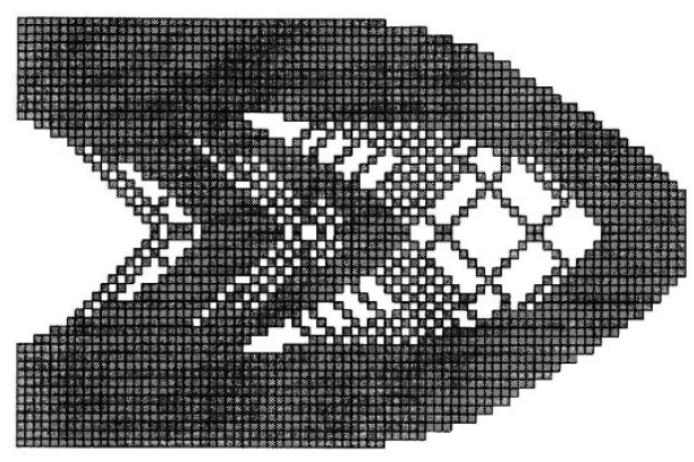
\includegraphics[scale=0.5]{Dissertation/images/chess.png} 
	\caption{Пример топологии <<шахматного поля>>}\label{fig:chess_topology}
\end{figure}

Для того чтобы избежать подобного результата используется сглаженная чувствительность элементов с фильтрацией, причем характерный размер фильтра $r_{min}$ не меняется с изменением сеточного разбиения. Величина $r_{min}$ создает круговую подобласть $\Omega_i$, центр которой совпадает с центром $i$-го элемента. Подобласть   накрывает несколько соседних элементов. Элементы, центры которых расположены внутри   создают вклад в сглаженную чувствительность $i$-го элемента согласно формуле

%\begin{equation}\label{eq:alpha}
%\begin{aligned}
%\alpha_i = \frac{\sum_{j=1}^K w(r_{ij}) \alpha_j^n}{K},
%\end{aligned}
%\end{equation}
\begin{equation}\label{eq:alpha}
	\begin{aligned}
		\alpha_i = \left(\sum_{j=1}^K w(r_{ij})) \alpha_j^n \right)/K,
	\end{aligned}
\end{equation}
где $K$~--- общее число узлов, содержащихся в подобласти $\Omega_i$, и $w(r_{ij})$~--- линейные веса, определяемые как

\begin{equation}\label{eq:w}
	\begin{aligned}
		w(r_{ij}) = \frac{r_{min}-r_{ij}}{K},
	\end{aligned}
\end{equation}

Таким образом, сглаживая значения чувствительности по всей области проектирования, схема фильтрации автоматически присваивает ненулевые значения чувствительности удаленным элементам. Для исключения значительных осцилляций минимизируемого функционала и резких изменений соответствующей топологии в итерационном процессе используется усреднение индексов чувствительности между текущим и предыдущим шагами оптимизации~\cite{Shevtsov2014}.

\begin{equation}\label{eq:w}
	\begin{aligned}
\alpha_i = \frac{\alpha_i^k - \alpha_i^{k+1}}{2},
	\end{aligned}
\end{equation}
где $k$~--- номер текущей итерации. На следующей итерации полагают $\alpha_i=\alpha_i^{k+1}$ и~т.~д. 

%Они внедрили схему фильтрации чувствительности, стабилизирующую процесс оптимизации с учетом истории изменений. Это позволило значительно расширить области применения метода, включая задачи оптимизации сложных конструкций с несколькими материалами.

Современные эволюционные методы подразделяются на две группы: подходы hard-kill и soft-kill. В hard-kill подходе материал удаляется полностью, что может вызвать проблемы со сходимостью метода. В soft-kill~\cite{Ghabraie2015}~--- удаление материала осуществляется плавно, через снижение модуля упругости элемента, что делает процесс оптимизации более стабильным и позволяет достичь высококачественных решений.

%Эволюционные методы продолжают активно развиваться, внедряются новые алгоритмы и расширяется их применение в различных задачах. Такие подходы остаются востребованными благодаря их гибкости, особенно при решении задач, требующих учета сложных физических ограничений и многоматериальных систем.













%%%%%%%%%%%%%%%%%%%%%%%%%%%%%%%%%%%%%%%%%%%%%%%%%%%%%%%%%%%%%%%%%%%%%%%%%%%%%%%%%%%%%%%%%

\section{Ссылки}\label{sec:ch1/sec2}

Мы можем сделать \textbf{жирный текст} и \textit{курсив}.

Сошлёмся на библиографию.
Одна ссылка: \cite[с.~54]{Sokolov}\cite[с.~36]{Gaidaenko}.
Две ссылки: \cite{Sokolov,Gaidaenko}.
Ссылка на собственные работы: \cite{vakbib1, confbib2}.
Много ссылок: %\cite[с.~54]{Lermontov,Management,Borozda} % такой «фокус»
%вызывает biblatex warning относительно опции sortcites, потому что неясно, к
%какому источнику относится уточнение о страницах, а bibtex об этой проблеме
%даже не предупреждает
\cite{Lermontov, Management, Borozda, Marketing, Constitution, FamilyCode,
    Gost.7.0.53, Razumovski, Lagkueva, Pokrovski, Methodology, Berestova,
    Kriger}%
\ifnumequal{\value{bibliosel}}{0}{% Примеры для bibtex8
    \cite{Sirotko, Lukina, Encyclopedia, Nasirova}%
}{% Примеры для biblatex через движок biber
    \cite{Sirotko2, Lukina2, Encyclopedia2, Nasirova2}%
}%
.
И~ещё немного ссылок:~\cite{Article,Book,Booklet,Conference,Inbook,Incollection,Manual,Mastersthesis,
    Misc,Phdthesis,Proceedings,Techreport,Unpublished}
% Следует обратить внимание, что пробел после запятой внутри \cite{}
% обрабатывается ожидаемо, а пробел перед запятой, может вызывать проблемы при
% обработке ссылок.
\cite{medvedev2006jelektronnye, CEAT:CEAT581, doi:10.1080/01932691.2010.513279,
    Gosele1999161,Li2007StressAnalysis, Shoji199895, test:eisner-sample,
    test:eisner-sample-shorted, AB_patent_Pomerantz_1968, iofis_patent1960}%
\ifnumequal{\value{bibliosel}}{0}{% Примеры для bibtex8
}{% Примеры для biblatex через движок biber
    \cite{patent2h, patent3h, patent2}%
}%
.

\ifnumequal{\value{bibliosel}}{0}{% Примеры для bibtex8
Попытка реализовать несколько ссылок на конкретные страницы
для \texttt{bibtex} реализации библиографии:
[\citenum{Sokolov}, с.~54; \citenum{Gaidaenko}, с.~36].
}{% Примеры для biblatex через движок biber
Несколько источников (мультицитата):
% Тут специально написано по-разному тире, для демонстрации, что
% применение специальных тире в настоящий момент в biblatex приводит к непоказу
% "с.".
\cites[vii--x, 5, 7]{Sokolov}[v"--~x, 25, 526]{Gaidaenko}[vii--x, 5, 7]{Techreport},
работает только в \texttt{biblatex} реализации библиографии.
}%

Ссылки на собственные работы:~\cite{vakbib1, confbib1}.

Сошлёмся на приложения: Приложение~\cref{app:A}, Приложение~\cref{app:B2}.

Сошлёмся на формулу: формула~\cref{eq:equation1}.

Сошлёмся на изображение: рисунок~\cref{fig:knuth}.

Стандартной практикой является добавление к ссылкам префикса, характеризующего тип элемента.
Это не является строгим требованием, но~позволяет лучше ориентироваться в документах большого размера.
Например, для ссылок на~рисунки используется префикс \textit{fig},
для ссылки на~таблицу "--- \textit{tab}.

В таблице \cref{tab:tab_pref} приложения~\cref{app:B4} приведён список рекомендуемых
к использованию стандартных префиксов.

В некоторых ситуациях возникает необходимость отойти от требований ГОСТ по оформлению ссылок на
литературу.
В таком случае можно воспользоваться дополнительными опциями пакета \verb+biblatex+.

Например, в ссылке на книгу~\cite{sobenin_kdv} использование опции \verb+maxnames=4+ позволяет
вывести имена всех четырёх авторов.
По ГОСТ имена последних трёх авторов опускаются.

Кроме того, часто возникают проблемы с транслитерованными инициалами. Некоторые буквы русского
алфавита по правилам транслитерации записываются двумя буквами латинского алфавита (ю-yu, ё-yo и
т.д.).
Такие инициалы \verb+biblatex+ будет сокращать до одной буквы, что неверно.
Поправить его работу можно использовав опцию \verb+giveninits=false+.
Пример использования этой опции можно видеть в ссылке~\cite{initials}.

\section{Формулы}\label{sec:ch1/sec3}

Благодаря пакету \textit{icomma}, \LaTeX~одинаково хорошо воспринимает
в~качестве десятичного разделителя и запятую (\(3,1415\)), и точку (\(3.1415\)).

\subsection{Ненумерованные одиночные формулы}\label{subsec:ch1/sec3/sub1}

Вот так может выглядеть формула, которую необходимо вставить в~строку
по~тексту: \(x \approx \sin x\) при \(x \to 0\).

А вот так выглядит ненумерованная отдельностоящая формула c подстрочными
и надстрочными индексами:
\[
    (x_1+x_2)^2 = x_1^2 + 2 x_1 x_2 + x_2^2
\]

Формула с неопределенным интегралом:
\[
    \int f(\alpha+x)=\sum\beta
\]

При использовании дробей формулы могут получаться очень высокие:
\[
    \frac{1}{\sqrt{2}+
        \displaystyle\frac{1}{\sqrt{2}+
            \displaystyle\frac{1}{\sqrt{2}+\cdots}}}
\]

В формулах можно использовать греческие буквы:
%Все \original... команды заранее, ради этого примера, определены в Dissertation\userstyles.tex
\[
    \alpha\beta\gamma\delta\originalepsilon\epsilon\zeta\eta\theta%
    \vartheta\iota\kappa\varkappa\lambda\mu\nu\xi\pi\varpi\rho\varrho%
    \sigma\varsigma\tau\upsilon\originalphi\phi\chi\psi\omega\Gamma\Delta%
    \Theta\Lambda\Xi\Pi\Sigma\Upsilon\Phi\Psi\Omega
\]
\[%https://texfaq.org/FAQ-boldgreek
    \boldsymbol{\alpha\beta\gamma\delta\originalepsilon\epsilon\zeta\eta%
        \theta\vartheta\iota\kappa\varkappa\lambda\mu\nu\xi\pi\varpi\rho%
        \varrho\sigma\varsigma\tau\upsilon\originalphi\phi\chi\psi\omega\Gamma%
        \Delta\Theta\Lambda\Xi\Pi\Sigma\Upsilon\Phi\Psi\Omega}
\]

Для добавления формул можно использовать пары \verb+$+\dots\verb+$+ и \verb+$$+\dots\verb+$$+,
но~они считаются устаревшими.
Лучше использовать их функциональные аналоги \verb+\(+\dots\verb+\)+ и \verb+\[+\dots\verb+\]+.

\subsection{Ненумерованные многострочные формулы}\label{subsec:ch1/sec3/sub2}

Вот так можно написать две формулы, не нумеруя их, чтобы знаки <<равно>> были
строго друг под другом:
\begin{align}
    f_W & =  \min \left( 1, \max \left( 0, \frac{W_{soil} / W_{max}}{W_{crit}} \right)  \right), \nonumber \\
    f_T & =  \min \left( 1, \max \left( 0, \frac{T_s / T_{melt}}{T_{crit}} \right)  \right), \nonumber
\end{align}

Выровнять систему ещё и по переменной \( x \) можно, используя окружение
\verb|alignedat| из пакета \verb|amsmath|. Вот так:
\[
|x| = \left\{
\begin{alignedat}{2}
     &   & x, \quad & \text{eсли } x\geqslant 0 \\
     & - & x, \quad & \text{eсли } x<0
\end{alignedat}
\right.
\]
Здесь первый амперсанд (в исходном \LaTeX\ описании формулы) означает
выравнивание по~левому краю, второй "--- по~\( x \), а~третий "--- по~слову
<<если>>. Команда \verb|\quad| делает большой горизонтальный пробел.

Ещё вариант:
\[
    |x|=
    \begin{cases}
        \phantom{-}x, \text{если } x \geqslant 0 \\
        -x, \text{если } x<0
    \end{cases}
\]

Кроме того, для  нумерованных формул \verb|alignedat| делает вертикальное
выравнивание номера формулы по центру формулы. Например, выравнивание
компонент вектора:
\begin{equation}
    \label{eq:2p3}
    \begin{alignedat}{2}
        {\mathbf{N}}_{o1n}^{(j)} = \,{\sin} \phi\,n\!\left(n+1\right)
        {\sin}\theta\,
        \pi_n\!\left({\cos} \theta\right)
        \frac{
        z_n^{(j)}\!\left( \rho \right)
        }{\rho}\,
         & {\boldsymbol{\hat{\mathrm e}}}_{r}\,+      \\
        +\,
        {\sin} \phi\,
        \tau_n\!\left({\cos} \theta\right)
        \frac{
        \left[\rho z_n^{(j)}\!\left( \rho \right)\right]^{\prime}
        }{\rho}\,
         & {\boldsymbol{\hat{\mathrm e}}}_{\theta}\,+ \\
        +\,
        {\cos} \phi\,
        \pi_n\!\left({\cos} \theta\right)
        \frac{
        \left[\rho z_n^{(j)}\!\left( \rho \right)\right]^{\prime}
        }{\rho}\,
         & {\boldsymbol{\hat{\mathrm e}}}_{\phi}\:.
    \end{alignedat}
\end{equation}

Ещё об отступах. Иногда для лучшей <<читаемости>> формул полезно
немного исправить стандартные интервалы \LaTeX\ с учётом логической
структуры самой формулы. Например в формуле~\cref{eq:2p3} добавлен
небольшой отступ \verb+\,+ между основными сомножителями, ниже
результат применения всех вариантов отступа:
\begin{align*}
    \backslash!             & \quad f(x) = x^2\! +3x\! +2         \\
    \mbox{по-умолчанию}     & \quad f(x) = x^2+3x+2               \\
    \backslash,             & \quad f(x) = x^2\, +3x\, +2         \\
    \backslash{:}           & \quad f(x) = x^2\: +3x\: +2         \\
    \backslash;             & \quad f(x) = x^2\; +3x\; +2         \\
    \backslash \mbox{space} & \quad f(x) = x^2\ +3x\ +2           \\
    \backslash \mbox{quad}  & \quad f(x) = x^2\quad +3x\quad +2   \\
    \backslash \mbox{qquad} & \quad f(x) = x^2\qquad +3x\qquad +2
\end{align*}

Можно использовать разные математические алфавиты:
\begin{align}
    \mathcal{ABCDEFGHIJKLMNOPQRSTUVWXYZ} \nonumber  \\
    \mathfrak{ABCDEFGHIJKLMNOPQRSTUVWXYZ} \nonumber \\
    \mathbb{ABCDEFGHIJKLMNOPQRSTUVWXYZ} \nonumber
\end{align}

Посмотрим на систему уравнений на примере аттрактора Лоренца:

\[
\left\{
\begin{array}{rl}
    \dot x = & \sigma (y-x)  \\
    \dot y = & x (r - z) - y \\
    \dot z = & xy - bz
\end{array}
\right.
\]

А для вёрстки матриц удобно использовать многоточия:
\[
    \left(
        \begin{array}{ccc}
            a_{11} & \ldots & a_{1n} \\
            \vdots & \ddots & \vdots \\
            a_{n1} & \ldots & a_{nn} \\
        \end{array}
    \right)
\]

\subsection{Нумерованные формулы}\label{subsec:ch1/sec3/sub3}

А вот так пишется нумерованная формула:
\begin{equation}
    \label{eq:equation1}
    e = \lim_{n \to \infty} \left( 1+\frac{1}{n} \right) ^n
\end{equation}

Нумерованных формул может быть несколько:
\begin{equation}
    \label{eq:equation2}
    \lim_{n \to \infty} \sum_{k=1}^n \frac{1}{k^2} = \frac{\pi^2}{6}
\end{equation}

Впоследствии на формулы~\cref{eq:equation1, eq:equation2} можно ссылаться.

Сделать так, чтобы номер формулы стоял напротив средней строки, можно,
используя окружение \verb|multlined| (пакет \verb|mathtools|) вместо
\verb|multline| внутри окружения \verb|equation|. Вот так:
\begin{equation} % \tag{S} % tag - вписывает свой текст
    \label{eq:equation3}
    \begin{multlined}
        1+ 2+3+4+5+6+7+\dots + \\
        + 50+51+52+53+54+55+56+57 + \dots + \\
        + 96+97+98+99+100=5050
    \end{multlined}
\end{equation}

Уравнения~\cref{eq:subeq_1,eq:subeq_2} демонстрируют возможности
окружения \verb|subequations| (пакет \verb|amsmath|).
\begin{subequations}
    \label{eq:subeq_1}
    \begin{gather}
        y = x^2 + 1 \label{eq:subeq_1-1} \\
        y = 2 x^2 - x + 1 \label{eq:subeq_1-2}
    \end{gather}
\end{subequations}
Ссылки на отдельные уравнения~\cref{eq:subeq_1-1,eq:subeq_1-2,eq:subeq_2-1}.
\begin{subequations}
    \label{eq:subeq_2}
    \begin{align}
        y & = x^3 + x^2 + x + 1 \label{eq:subeq_2-1} \\
        y & = x^2
    \end{align}
\end{subequations}

\subsection{Форматирование чисел и размерностей величин}\label{sec:units}

Числа форматируются при помощи команды \verb|\num|:
\num{5,3};
\num{2,3e8};
\num{12345,67890};
\num{2,6 d4};
\num{1+-2i};
\num{.3e45};
\num[exponent-base=2]{5 e64};
\num[exponent-base=2,exponent-to-prefix]{5 e64};
\num{1.654 x 2.34 x 3.430}
\num{1 2 x 3 / 4}.
Для написания последовательности чисел можно использовать команды \verb|\numlist| и \verb|\numrange|:
\numlist{10;30;50;70}; \numrange{10}{30}.
Значения углов можно форматировать при помощи команды \verb|\ang|:
\ang{2.67};
\ang{30,3};
\ang{-1;;};
\ang{;-2;};
\ang{;;-3};
\ang{300;10;1}.

Обратите внимание, что ГОСТ запрещает использование знака <<->> для обозначения отрицательных чисел
за исключением формул, таблиц и~рисунков.
Вместо него следует использовать слово <<минус>>.

Размерности можно записывать при помощи команд \verb|\si| и \verb|\SI|:
\si{\farad\squared\lumen\candela};
\si{\joule\per\mole\per\kelvin};
\si[per-mode = symbol-or-fraction]{\joule\per\mole\per\kelvin};
\si{\metre\per\second\squared};
\SI{0.10(5)}{\neper};
\SI{1.2-3i e5}{\joule\per\mole\per\kelvin};
\SIlist{1;2;3;4}{\tesla};
\SIrange{50}{100}{\volt}.
Список единиц измерений приведён в таблицах~\cref{tab:unit:base,
    tab:unit:derived,tab:unit:accepted,tab:unit:physical,tab:unit:other}.
Приставки единиц приведены в~таблице~\cref{tab:unit:prefix}.

С дополнительными опциями форматирования можно ознакомиться в~описании пакета \texttt{siunitx};
изменить или добавить единицы измерений можно в~файле \texttt{siunitx.cfg}.

\begin{table}
    \centering
    \captionsetup{justification=centering} % выравнивание подписи по-центру
    \caption{Основные величины СИ}\label{tab:unit:base}
    \begin{tabular}{llc}
        \toprule
        Название  & Команда          & Символ         \\
        \midrule
        Ампер     & \verb|\ampere|   & \si{\ampere}   \\
        Кандела   & \verb|\candela|  & \si{\candela}  \\
        Кельвин   & \verb|\kelvin|   & \si{\kelvin}   \\
        Килограмм & \verb|\kilogram| & \si{\kilogram} \\
        Метр      & \verb|\metre|    & \si{\metre}    \\
        Моль      & \verb|\mole|     & \si{\mole}     \\
        Секунда   & \verb|\second|   & \si{\second}   \\
        \bottomrule
    \end{tabular}
\end{table}

\begin{table}
    \small
    \centering
    \begin{threeparttable}% выравнивание подписи по границам таблицы
        \caption{Производные единицы СИ}\label{tab:unit:derived}
        \begin{tabular}{llc|llc}
            \toprule
            Название       & Команда               & Символ              & Название & Команда & Символ \\
            \midrule
            Беккерель      & \verb|\becquerel|     & \si{\becquerel}     &
            Ньютон         & \verb|\newton|        & \si{\newton}                                      \\
            Градус Цельсия & \verb|\degreeCelsius| & \si{\degreeCelsius} &
            Ом             & \verb|\ohm|           & \si{\ohm}                                         \\
            Кулон          & \verb|\coulomb|       & \si{\coulomb}       &
            Паскаль        & \verb|\pascal|        & \si{\pascal}                                      \\
            Фарад          & \verb|\farad|         & \si{\farad}         &
            Радиан         & \verb|\radian|        & \si{\radian}                                      \\
            Грей           & \verb|\gray|          & \si{\gray}          &
            Сименс         & \verb|\siemens|       & \si{\siemens}                                     \\
            Герц           & \verb|\hertz|         & \si{\hertz}         &
            Зиверт         & \verb|\sievert|       & \si{\sievert}                                     \\
            Генри          & \verb|\henry|         & \si{\henry}         &
            Стерадиан      & \verb|\steradian|     & \si{\steradian}                                   \\
            Джоуль         & \verb|\joule|         & \si{\joule}         &
            Тесла          & \verb|\tesla|         & \si{\tesla}                                       \\
            Катал          & \verb|\katal|         & \si{\katal}         &
            Вольт          & \verb|\volt|          & \si{\volt}                                        \\
            Люмен          & \verb|\lumen|         & \si{\lumen}         &
            Ватт           & \verb|\watt|          & \si{\watt}                                        \\
            Люкс           & \verb|\lux|           & \si{\lux}           &
            Вебер          & \verb|\weber|         & \si{\weber}                                       \\
            \bottomrule
        \end{tabular}
    \end{threeparttable}
\end{table}

\begin{table}
    \centering
    \begin{threeparttable}% выравнивание подписи по границам таблицы
        \caption{Внесистемные единицы}\label{tab:unit:accepted}

        \begin{tabular}{llc}
            \toprule
            Название        & Команда           & Символ          \\
            \midrule
            День            & \verb|\day|       & \si{\day}       \\
            Градус          & \verb|\degree|    & \si{\degree}    \\
            Гектар          & \verb|\hectare|   & \si{\hectare}   \\
            Час             & \verb|\hour|      & \si{\hour}      \\
            Литр            & \verb|\litre|     & \si{\litre}     \\
            Угловая минута  & \verb|\arcminute| & \si{\arcminute} \\
            Угловая секунда & \verb|\arcsecond| & \si{\arcsecond} \\ %
            Минута          & \verb|\minute|    & \si{\minute}    \\
            Тонна           & \verb|\tonne|     & \si{\tonne}     \\
            \bottomrule
        \end{tabular}
    \end{threeparttable}
\end{table}

\begin{table}
    \centering
    \captionsetup{justification=centering}
    \caption{Внесистемные единицы, получаемые из эксперимента}\label{tab:unit:physical}
    \begin{tabular}{llc}
        \toprule
        Название                & Команда                  & Символ                 \\
        \midrule
        Астрономическая единица & \verb|\astronomicalunit| & \si{\astronomicalunit} \\
        Атомная единица массы   & \verb|\atomicmassunit|   & \si{\atomicmassunit}   \\
        Боровский радиус        & \verb|\bohr|             & \si{\bohr}             \\
        Скорость света          & \verb|\clight|           & \si{\clight}           \\
        Дальтон                 & \verb|\dalton|           & \si{\dalton}           \\
        Масса электрона         & \verb|\electronmass|     & \si{\electronmass}     \\
        Электрон Вольт          & \verb|\electronvolt|     & \si{\electronvolt}     \\
        Элементарный заряд      & \verb|\elementarycharge| & \si{\elementarycharge} \\
        Энергия Хартри          & \verb|\hartree|          & \si{\hartree}          \\
        Постоянная Планка       & \verb|\planckbar|        & \si{\planckbar}        \\
        \bottomrule
    \end{tabular}
\end{table}

\begin{table}
    \centering
    \begin{threeparttable}% выравнивание подписи по границам таблицы
        \caption{Другие внесистемные единицы}\label{tab:unit:other}
        \begin{tabular}{llc}
            \toprule
            Название                  & Команда              & Символ             \\
            \midrule
            Ангстрем                  & \verb|\angstrom|     & \si{\angstrom}     \\
            Бар                       & \verb|\bar|          & \si{\bar}          \\
            Барн                      & \verb|\barn|         & \si{\barn}         \\
            Бел                       & \verb|\bel|          & \si{\bel}          \\
            Децибел                   & \verb|\decibel|      & \si{\decibel}      \\
            Узел                      & \verb|\knot|         & \si{\knot}         \\
            Миллиметр ртутного столба & \verb|\mmHg|         & \si{\mmHg}         \\
            Морская миля              & \verb|\nauticalmile| & \si{\nauticalmile} \\
            Непер                     & \verb|\neper|        & \si{\neper}        \\
            \bottomrule
        \end{tabular}
    \end{threeparttable}
\end{table}

\begin{table}
    \small
    \centering
    \begin{threeparttable}% выравнивание подписи по границам таблицы
        \caption{Приставки СИ}\label{tab:unit:prefix}
        \begin{tabular}{llcc|llcc}
            \toprule
            Приставка & Команда       & Символ      & Степень      &
            Приставка & Команда       & Символ      & Степень        \\
            \midrule
            Иокто     & \verb|\yocto| & \si{\yocto} & \textminus24 &
            Дека      & \verb|\deca|  & \si{\deca}  & 1              \\
            Зепто     & \verb|\zepto| & \si{\zepto} & \textminus21 &
            Гекто     & \verb|\hecto| & \si{\hecto} & 2              \\
            Атто      & \verb|\atto|  & \si{\atto}  & \textminus18 &
            Кило      & \verb|\kilo|  & \si{\kilo}  & 3              \\
            Фемто     & \verb|\femto| & \si{\femto} & \textminus15 &
            Мега      & \verb|\mega|  & \si{\mega}  & 6              \\
            Пико      & \verb|\pico|  & \si{\pico}  & \textminus12 &
            Гига      & \verb|\giga|  & \si{\giga}  & 9              \\
            Нано      & \verb|\nano|  & \si{\nano}  & \textminus9  &
            Терра     & \verb|\tera|  & \si{\tera}  & 12             \\
            Микро     & \verb|\micro| & \si{\micro} & \textminus6  &
            Пета      & \verb|\peta|  & \si{\peta}  & 15             \\
            Милли     & \verb|\milli| & \si{\milli} & \textminus3  &
            Екса      & \verb|\exa|   & \si{\exa}   & 18             \\
            Санти     & \verb|\centi| & \si{\centi} & \textminus2  &
            Зетта     & \verb|\zetta| & \si{\zetta} & 21             \\
            Деци      & \verb|\deci|  & \si{\deci}  & \textminus1  &
            Иотта     & \verb|\yotta| & \si{\yotta} & 24             \\
            \bottomrule
        \end{tabular}
    \end{threeparttable}
\end{table}

\subsection{Заголовки с формулами: \texorpdfstring{\(a^2 + b^2 = c^2\)}{%
        a\texttwosuperior\ + b\texttwosuperior\ = c\texttwosuperior},
    \texorpdfstring{\(\left\vert\textrm{{Im}}\Sigma\left(
            \protect\varepsilon\right)\right\vert\approx const\)}{|ImΣ (ε)| ≈ const},
    \texorpdfstring{\(\sigma_{xx}^{(1)}\)}{σ\_\{xx\}\textasciicircum\{(1)\}}
}\label{subsec:with_math}

Пакет \texttt{hyperref} берёт текст для закладок в pdf-файле из~аргументов
команд типа \verb|\section|, которые могут содержать математические формулы,
а~также изменения цвета текста или шрифта, которые не отображаются в~закладках.
Чтобы использование формул в заголовках не вызывало в~логе компиляции появление
предупреждений типа <<\texttt{Token not allowed in~a~PDF string
    (Unicode):(hyperref) removing...}>>, следует использовать конструкцию
\verb|\texorpdfstring{}{}|, где в~первых фигурных скобках указывается
формула, а~во~вторых "--- запись формулы для закладок.

%\replace{text}{replacement}\section{Рецензирование текста}\label{sec:markup}

В шаблоне для диссертации и автореферата заданы команды рецензирования.
Они видны при компиляции шаблона в режиме черновика или при установке
соответствующей настройки (\verb+showmarkup+) в~файле \verb+common/setup.tex+.

Команда \verb+\todo+ отмечает текст красным цветом.
\todo{Например, так.}

Команда \verb+\note+ позволяет выбрать цвет текста.
\note{Чёрный, } \note[red]{красный, } \note[green]{зелёный, }
\note[blue]{синий.} \note[orange]{Обратите внимание на ширину и расстановку
    формирующихся пробелов, в~результате приведённой записи (зависит также
    от~применяемого компилятора).}

Окружение \verb+commentbox+ также позволяет выбрать цвет.

\begin{commentbox}[red]
    Красный текст.

    Несколько параграфов красного текста.
\end{commentbox}

\begin{commentbox}[blue]
    Синяя формула.

    \begin{equation}
        \alpha + \beta = \gamma
    \end{equation}
\end{commentbox}

\verb+commentbox+ позволяет закомментировать участок кода в~режиме чистовика.
Чтобы убрать кусок кода для всех режимов, можно использовать окружение
\verb+comment+.

\begin{comment}
Этот текст всегда скрыт.
\end{comment}

\section{Работа со списком сокращений и~условных обозначений}\label{sec:acronyms}

С помощью пакета \texttt{nomencl} можно создавать удобный сортированный список
сокращений и условных обозначений во время написания текста. Вызов
\verb+\nomenclature+ добавляет нужный символ или сокращение с~описанием
в~список, который затем печатается вызовом \verb+\printnomenclature+
в~соответствующем разделе.
Для того, чтобы эти операции прошли, потребуется дополнительный вызов
\verb+makeindex -s nomencl.ist -o %.nls %.nlo+ в~командной строке, где вместо
\verb+%+ следует подставить имя главного файла проекта (\verb+dissertation+
для этого шаблона).
Затем потребуется один или два дополнительных вызова компилятора проекта.
\begin{equation}
    \omega = c k,
\end{equation}
где \( \omega \) "--- частота света, \( c \) "--- скорость света, \( k \) "---
модуль волнового вектора.
\nomenclature{\(\omega\)}{частота света\nomrefeq}
\nomenclature{\(c\)}{скорость света\nomrefpage}
\nomenclature{\(k\)}{модуль волнового вектора\nomrefeqpage}
Использование
\begin{verbatim}
\nomenclature{\(\omega\)}{частота света\nomrefeq}
\nomenclature{\(c\)}{скорость света\nomrefpage}
\nomenclature{\(k\)}{модуль волнового вектора\nomrefeqpage}
\end{verbatim}
после уравнения добавит в список условных обозначений три записи.
Ссылки \verb+\nomrefeq+ на последнее уравнение, \verb+\nomrefpage+ "--- на
страницу, \verb+\nomrefeqpage+ "--- сразу на~последнее уравнение и~на~страницу,
можно опускать и~не~использовать.

Группировкой и сортировкой пунктов в списке можно управлять с~помощью указания
дополнительных аргументов к команде \verb+nomenclature+.
Например, при вызове
\begin{verbatim}
\nomenclature[03]{\( \hbar \)}{постоянная Планка}
\nomenclature[01]{\( G \)}{гравитационная постоянная}
\end{verbatim}
\( G \) будет стоять в списке выше, чем \( \hbar \).
Для корректных вертикальных отступов между строками в описании лучше
не~использовать многострочные формулы в~списке обозначений.

\nomenclature{%
    \( \begin{rcases}
        a_n \\
        b_n
    \end{rcases} \)%
}{коэффициенты разложения Ми в дальнем поле соответствующие электрическим и
    магнитным мультиполям}
\nomenclature[a\( e \)]{\( {\boldsymbol{\hat{\mathrm e}}} \)}{единичный вектор}
\nomenclature{\( E_0 \)}{амплитуда падающего поля}
\nomenclature{\( j \)}{тип функции Бесселя}
\nomenclature{\( k \)}{волновой вектор падающей волны}
\nomenclature{%
    \( \begin{rcases}
        a_n \\
        b_n
    \end{rcases} \)%
}{и снова коэффициенты разложения Ми в дальнем поле соответствующие
    электрическим и магнитным мультиполям. Добавлено много текста, так что
    описание группы условных обозначений значительно превысило высоту этой
    группы...}
\nomenclature{\( L \)}{общее число слоёв}
\nomenclature{\( l \)}{номер слоя внутри стратифицированной сферы}
\nomenclature{\( \lambda \)}{длина волны электромагнитного излучения в вакууме}
\nomenclature{\( n \)}{порядок мультиполя}
\nomenclature{%
    \( \begin{rcases}
        {\mathbf{N}}_{e1n}^{(j)} & {\mathbf{N}}_{o1n}^{(j)} \\
        {\mathbf{M}_{o1n}^{(j)}} & {\mathbf{M}_{e1n}^{(j)}}
    \end{rcases} \)%
}{сферические векторные гармоники}
\nomenclature{\( \mu \)}{магнитная проницаемость в вакууме}
\nomenclature{\( r, \theta, \phi \)}{полярные координаты}
\nomenclature{\( \omega \)}{частота падающей волны}

С помощью \verb+nomenclature+ можно включать в~список сокращения,
не~используя их~в~тексте.
% запись сокращения в список происходит командой \nomenclature,
% а не употреблением самого сокращения
\nomenclature{FEM}{finite element method, метод конечных элементов}
\nomenclature{FIT}{finite integration technique, метод конечных интегралов}
\nomenclature{FMM}{fast multipole method, быстрый метод многополюсника}
\nomenclature{FVTD}{finite volume time-domain, метод конечных объёмов
    во~временной области}
\nomenclature{MLFMA}{multilevel fast multipole algorithm, многоуровневый
    быстрый алгоритм многополюсника}
\nomenclature{BEM}{boundary element method, метод граничных элементов}
\nomenclature{CST MWS}{Computer Simulation Technology Microwave Studio
    программа для компьютерного моделирования уравнен Максвелла}
\nomenclature{DDA}{discrete dipole approximation, приближение дискретиных
    диполей}
\nomenclature{FDFD}{finite difference frequency domain, метод конечных
    разностей в~частотной области}
\nomenclature{FDTD}{finite difference time domain, метод конечных разностей
    во~временной области}
\nomenclature{MoM}{method of moments, метод моментов}
\nomenclature{MSTM}{multiple sphere T-Matrix, метод Т-матриц для множества
    сфер}
\nomenclature{PSTD}{pseudospectral time domain method, псевдоспектральный метод
    во~временной области}
\nomenclature{TLM}{transmission line matrix method, метод матриц линий передач}

\FloatBarrier
